\documentclass{article}
\usepackage[utf8]{inputenc}
\usepackage{graphicx}
\usepackage[spanish]{babel}
\usepackage{amsmath}
\usepackage{amsfonts}
\usepackage{amssymb}
\usepackage{multicol}
\usepackage{multirow}
\usepackage{bigstrut}
\usepackage{booktabs}
\usepackage{caption}
\usepackage[left=2.54cm,right=2.54cm,top=2.54cm,bottom=2.54cm]{geometry}
\spanishdecimal{.}
\begin{document}
\begin{center} \LARGE{ESCUELA POLITECNICA NACIONAL} \\[0.5cm] \Large{FACULTAD DE INGENIERÍA EN SISTEMAS}\\[0.5cm] \large{PROBABILIDAD Y ESTADISTICA} \end{center}
\begin{figure}[htb] \centering 
\includegraphics[scale=.6]{descarga (1).png}\end{figure}
\begin{center} \large{\bf Proyecto 2° Bimestre:}\\ \vspace{.25cm} { \Large \bfseries \underline{UN CLIMA SABOR A CAFÉ}} \\ \end{center}
\large{\bf Estudiantes: Rafael Alexander Piedra Granda }\\
\large{\bf Docente: Monica Mantilla }\\
\large{\bf Grupo: }\\\begin{center} \Large \textsc{Quito - Ecuador} \\
\Large \textsc{2022}
\end{center}
\section{Introduccion}
\section{Metodologia}
\section{Resultados}
\begin{enumerate}
    \item Establezca un modelo de regresión lineal, el coeficiente de correlación y la interpretación correspondiente, que establezca la relación entre las ventas totales y la temperatura máxima diaria.
          \begin{center}
              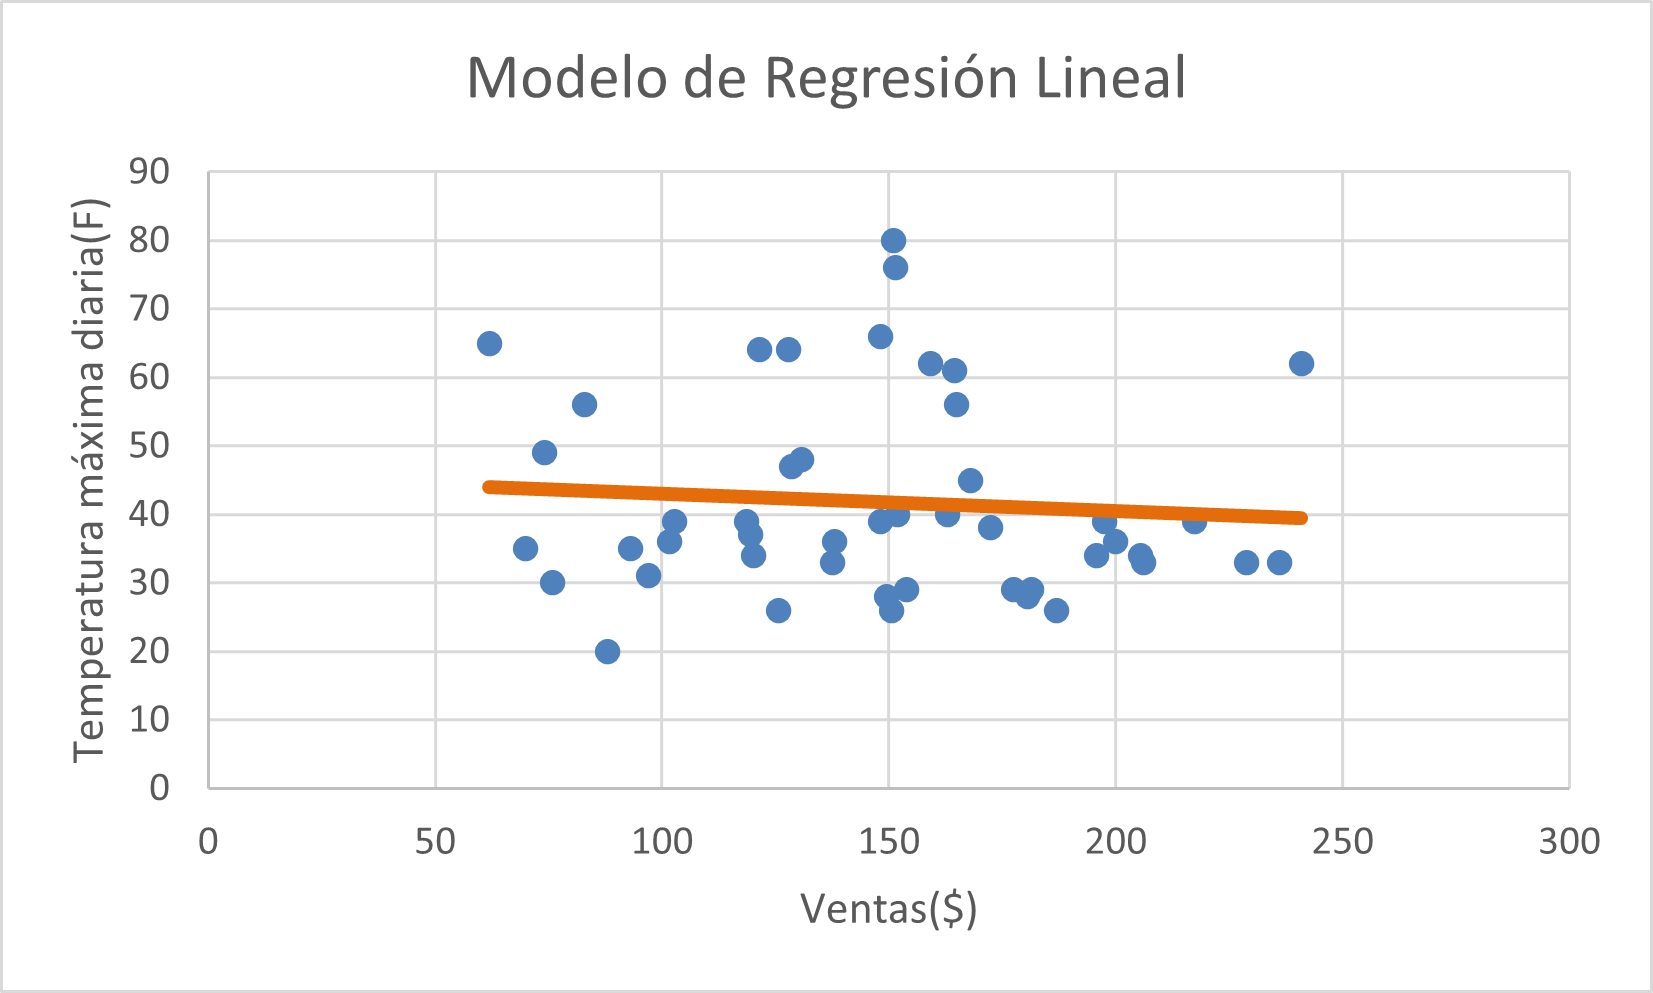
\includegraphics[width=\textwidth]{Imagen1.png}
              % \caption{Fig.1 Modelo de Regresión Lineal}
          \end{center}
    \item Determine un intervalo de confianza para la media y la varianza para el producto que más se desperdicia, con un nivel de confianza del 98%.
    \paragraph{}En un estudio previo se determinó que el producto que mas se vendió fueron los wraps, a continuación se determinan los intervalos de confianza para el producto.
    se tomó la siguiente muestra:\\
    % Table generated by Excel2LaTeX from sheet 'pregunta 2'
\begin{table}[htbp]
    \centering
    \caption{muestra aleatoria}
      \begin{tabular}{|c|c|c|c|c|c|c|c|}
      \toprule
      1     & 3     & 0     & 0     & 0     & 0     & 3     & 7 \\
      \midrule
      0     & 5     & 4     & 9     & 2     & 0     & 0     & 0 \\
      \bottomrule
      \end{tabular}%
    \label{tab:addlabel}%
  \end{table}%
   
    \begin{enumerate}{}
       
        \item{intervalo de confianza para la media}
            \paragraph{}Se tiene que $\bar{x}=2.125$, $n=16$ y $\sigma=7.61$.\\
            Debido a que estamos trabajando con un nivel de confianza del 98\%, por lo tanto se tiene que:\\ 
            $1-\alpha=0.98$, de donde $\alpha=0.02 $ y $\alpha/2=0.01$, por lo tanto, $z_{0.01}=2.33$ 
            Se tiene que el intervalo resultante es: \\\\
            $(\bar{x}-z_{\alpha/2}\frac{\sigma}{\sqrt{n}};\bar{x}+z_{\alpha/2}\frac{\sigma}{\sqrt{n}})=(3.73,21.83)$\\\\
            por lo tanto, tenemos que: $\mu$ $\epsilon$ $(3.73,21.83)$ con un 98\% de confianza
        

        \item {intervalo de confianza para la varianza}
        \paragraph{} A partir de los datos se tiene que $s^2=7.61$,$n=16$ y $1-\alpha=0.98$, ademas a partir de la tabla de la distribución chi-cuadrado con 15 grados de libertad se tiene que: \\\\
        $x_{0.01}^2=30.5779$ y $x_{0.99}^2=5.2294$ \\\\
        Por lo tanto el intervalo de confianza es: $(\frac{(n-1)s^2}{x_{\alpha/2}^2(n-1)};\frac{(n-1)s^2}{x_{1-\alpha/2}^2(n-1)})=(3.73;21.83)$ 
        
    \end{enumerate}   
    \item Determine un intervalo de confianza para la media y la varianza para la copa de frutas, con un nivel de confianza del 98%.
    % Table generated by Excel2LaTeX from sheet 'pregunta 3'
\begin{table}[htbp]
    \centering
    \caption{Add caption}
      \begin{tabular}{|c|c|c|c|c|c|c|c|}
      \toprule
      1     & 4     & 3     & 2     & 1     & 2     & 2     & 2 \\
      \midrule
      2     & 4     & 2     & 0     & 2     & 1     & 0     & 2 \\
      \bottomrule
      \end{tabular}%
    \label{tab:addlabel}%
  \end{table}%
  
    \begin{enumerate}{}
       
        \item{intervalo de confianza para la media}
            \paragraph{}Se tiene que $\bar{x}=1.875$, $n=16$ y $\sigma=1.15$.\\
            Debido a que estamos trabajando con un nivel de confianza del 98\%, por lo tanto se tiene que:\\ 
            $1-\alpha=0.98$, de donde $\alpha=0.02 $ y $\alpha/2=0.01$, por lo tanto, $z_{0.01}=2.33$ 
            Se tiene que el intervalo resultante es: \\\\
            $(\bar{x}-z_{\alpha/2}\frac{\sigma}{\sqrt{n}};\bar{x}+z_{\alpha/2}\frac{\sigma}{\sqrt{n}})=(1.21,2.54)$\\\\
            por lo tanto, tenemos que: $\mu$ $\epsilon$ $(1.21,2.54)$ con un 98\% de confianza
        
        \item {intervalo de confianza para la varianza}
        \paragraph{}
    \end{enumerate}
    \item Determine un intervalo de confianza para la media y la varianza para los tres productos más vendidos, con un nivel de confianza del 98%.
    \paragraph*{}\textbf{sodas}\\
    \begin{enumerate}{}
       
      \item{intervalo de confianza para la media}
          \paragraph{}Se tiene que $\bar{x}=1.875$, $n=16$ y $\sigma=1.15$.\\
          Debido a que estamos trabajando con un nivel de confianza del 98\%, por lo tanto se tiene que:\\ 
          $1-\alpha=0.98$, de donde $\alpha=0.02 $ y $\alpha/2=0.01$, por lo tanto, $z_{0.01}=2.33$ 
          Se tiene que el intervalo resultante es: \\\\
          $(\bar{x}-z_{\alpha/2}\frac{\sigma}{\sqrt{n}};\bar{x}+z_{\alpha/2}\frac{\sigma}{\sqrt{n}})=(1.21,2.54)$\\\\
          por lo tanto, tenemos que: $\mu$ $\epsilon$ $(1.21,2.54)$ con un 98\% de confianza
      
      \item {intervalo de confianza para la varianza}
      \paragraph{}
  \end{enumerate}
  \paragraph*{}\textbf{cafes}\\
    \begin{enumerate}{}
       
      \item{intervalo de confianza para la media}
          \paragraph{}Se tiene que $\bar{x}=1.875$, $n=16$ y $\sigma=1.15$.\\
          Debido a que estamos trabajando con un nivel de confianza del 98\%, por lo tanto se tiene que:\\ 
          $1-\alpha=0.98$, de donde $\alpha=0.02 $ y $\alpha/2=0.01$, por lo tanto, $z_{0.01}=2.33$ 
          Se tiene que el intervalo resultante es: \\\\
          $(\bar{x}-z_{\alpha/2}\frac{\sigma}{\sqrt{n}};\bar{x}+z_{\alpha/2}\frac{\sigma}{\sqrt{n}})=(1.21,2.54)$\\\\
          por lo tanto, tenemos que: $\mu$ $\epsilon$ $(1.21,2.54)$ con un 98\% de confianza
      
      \item {intervalo de confianza para la varianza}
      \paragraph{}
  \end{enumerate}
  \paragraph*{}\textbf{wraps}\\
    \begin{enumerate}{}
       
      \item{intervalo de confianza para la media}
          \paragraph{}Se tiene que $\bar{x}=1.875$, $n=16$ y $\sigma=1.15$.\\
          Debido a que estamos trabajando con un nivel de confianza del 98\%, por lo tanto se tiene que:\\ 
          $1-\alpha=0.98$, de donde $\alpha=0.02 $ y $\alpha/2=0.01$, por lo tanto, $z_{0.01}=2.33$ 
          Se tiene que el intervalo resultante es: \\\\
          $(\bar{x}-z_{\alpha/2}\frac{\sigma}{\sqrt{n}};\bar{x}+z_{\alpha/2}\frac{\sigma}{\sqrt{n}})=(1.21,2.54)$\\\\
          por lo tanto, tenemos que: $\mu$ $\epsilon$ $(1.21,2.54)$ con un 98\% de confianza
      
      \item {intervalo de confianza para la varianza}
      \paragraph{}
  \end{enumerate}

    % \begin{enumerate}
    %   \item{sodas}
    %   \item{wraps}
    %   \item{colas} 
    % \end{enumerate}
    \item Determine una prueba de hipótesis para la media, la varianza y la proporción para el número de tazas de café que se venden por día, con un nivel de confianza del 98%
    \item Determine una prueba de hipótesis para la media, la varianza y la proporción para el total de ventas, con un nivel de confianza del 98%
\end{enumerate}
\section{Análisis}
\section{Apéndices}
\section{Referencias}
\end{document}